\documentclass[]{article}
\usepackage[left=1in,top=1in,right=1in,bottom=1in]{geometry}


%%%% more monte %%%%
% thispagestyle{empty}
% https://stackoverflow.com/questions/2166557/how-to-hide-the-page-number-in-latex-on-first-page-of-a-chapter
\usepackage{color}
% \usepackage[table]{xcolor} % are they using color?

% \definecolor{WSU.crimson}{HTML}{981e32}
% \definecolor{WSU.gray}{HTML}{5e6a71}

% \definecolor{shadecolor}{RGB}{248,248,248}
\definecolor{WSU.crimson}{RGB}{152,30,50} % use http://colors.mshaffer.com to convert from 981e32
\definecolor{WSU.gray}{RGB}{94,106,113}

%%%%%%%%%%%%%%%%%%%%%%%%%%%%

\newcommand*{\authorfont}{\fontfamily{phv}\selectfont}
\usepackage{lmodern}


  \usepackage[T1]{fontenc}
  \usepackage[utf8]{inputenc}




\usepackage{abstract}
\renewcommand{\abstractname}{}    % clear the title
\renewcommand{\absnamepos}{empty} % originally center

\renewenvironment{abstract}
 {{%
    \setlength{\leftmargin}{0mm}
    \setlength{\rightmargin}{\leftmargin}%
  }%
  \relax}
 {\endlist}

\makeatletter
\def\@maketitle{%
  \pagestyle{empty}
  \newpage
%  \null
%  \vskip 2em%
%  \begin{center}%
  \let \footnote \thanks
    {\fontsize{18}{20}\selectfont\raggedright  \setlength{\parindent}{0pt} \@title \par}%
}
%\fi
\makeatother






\usepackage{color}
\usepackage{fancyvrb}
\newcommand{\VerbBar}{|}
\newcommand{\VERB}{\Verb[commandchars=\\\{\}]}
\DefineVerbatimEnvironment{Highlighting}{Verbatim}{commandchars=\\\{\}}
% Add ',fontsize=\small' for more characters per line
\usepackage{framed}
\definecolor{shadecolor}{RGB}{248,248,248}
\newenvironment{Shaded}{\begin{snugshade}}{\end{snugshade}}
\newcommand{\AlertTok}[1]{\textcolor[rgb]{0.94,0.16,0.16}{#1}}
\newcommand{\AnnotationTok}[1]{\textcolor[rgb]{0.56,0.35,0.01}{\textbf{\textit{#1}}}}
\newcommand{\AttributeTok}[1]{\textcolor[rgb]{0.77,0.63,0.00}{#1}}
\newcommand{\BaseNTok}[1]{\textcolor[rgb]{0.00,0.00,0.81}{#1}}
\newcommand{\BuiltInTok}[1]{#1}
\newcommand{\CharTok}[1]{\textcolor[rgb]{0.31,0.60,0.02}{#1}}
\newcommand{\CommentTok}[1]{\textcolor[rgb]{0.56,0.35,0.01}{\textit{#1}}}
\newcommand{\CommentVarTok}[1]{\textcolor[rgb]{0.56,0.35,0.01}{\textbf{\textit{#1}}}}
\newcommand{\ConstantTok}[1]{\textcolor[rgb]{0.00,0.00,0.00}{#1}}
\newcommand{\ControlFlowTok}[1]{\textcolor[rgb]{0.13,0.29,0.53}{\textbf{#1}}}
\newcommand{\DataTypeTok}[1]{\textcolor[rgb]{0.13,0.29,0.53}{#1}}
\newcommand{\DecValTok}[1]{\textcolor[rgb]{0.00,0.00,0.81}{#1}}
\newcommand{\DocumentationTok}[1]{\textcolor[rgb]{0.56,0.35,0.01}{\textbf{\textit{#1}}}}
\newcommand{\ErrorTok}[1]{\textcolor[rgb]{0.64,0.00,0.00}{\textbf{#1}}}
\newcommand{\ExtensionTok}[1]{#1}
\newcommand{\FloatTok}[1]{\textcolor[rgb]{0.00,0.00,0.81}{#1}}
\newcommand{\FunctionTok}[1]{\textcolor[rgb]{0.00,0.00,0.00}{#1}}
\newcommand{\ImportTok}[1]{#1}
\newcommand{\InformationTok}[1]{\textcolor[rgb]{0.56,0.35,0.01}{\textbf{\textit{#1}}}}
\newcommand{\KeywordTok}[1]{\textcolor[rgb]{0.13,0.29,0.53}{\textbf{#1}}}
\newcommand{\NormalTok}[1]{#1}
\newcommand{\OperatorTok}[1]{\textcolor[rgb]{0.81,0.36,0.00}{\textbf{#1}}}
\newcommand{\OtherTok}[1]{\textcolor[rgb]{0.56,0.35,0.01}{#1}}
\newcommand{\PreprocessorTok}[1]{\textcolor[rgb]{0.56,0.35,0.01}{\textit{#1}}}
\newcommand{\RegionMarkerTok}[1]{#1}
\newcommand{\SpecialCharTok}[1]{\textcolor[rgb]{0.00,0.00,0.00}{#1}}
\newcommand{\SpecialStringTok}[1]{\textcolor[rgb]{0.31,0.60,0.02}{#1}}
\newcommand{\StringTok}[1]{\textcolor[rgb]{0.31,0.60,0.02}{#1}}
\newcommand{\VariableTok}[1]{\textcolor[rgb]{0.00,0.00,0.00}{#1}}
\newcommand{\VerbatimStringTok}[1]{\textcolor[rgb]{0.31,0.60,0.02}{#1}}
\newcommand{\WarningTok}[1]{\textcolor[rgb]{0.56,0.35,0.01}{\textbf{\textit{#1}}}}



\title{\textbf{\textcolor{WSU.crimson}{What can body composition data
tell us?}} \newline \textbf{\textcolor{WSU.gray}{How are diffeerent
measurements related?}}  }
 

%  

% \author{ \Large true \hfill \normalsize \emph{} }
\author{\Large Michaela
Bayerlova\vspace{0.05in} \newline\normalsize\emph{Washington State
University}  }


\date{November 16, 2020}
\setcounter{secnumdepth}{3}

\usepackage{titlesec}
% See the link above: KOMA classes are not compatible with titlesec any more. Sorry.
% https://github.com/jbezos/titlesec/issues/11
\titleformat*{\section}{\bfseries}
\titleformat*{\subsection}{\bfseries\itshape}
\titleformat*{\subsubsection}{\itshape}
\titleformat*{\paragraph}{\itshape}
\titleformat*{\subparagraph}{\itshape}

% https://code.usgs.gov/usgs/norock/irvine_k/ip-092225/


%\titleformat*{\section}{\normalsize\bfseries}
%\titleformat*{\subsection}{\normalsize\itshape}
%\titleformat*{\subsubsection}{\normalsize\itshape}
%\titleformat*{\paragraph}{\normalsize\itshape}
%\titleformat*{\subparagraph}{\normalsize\itshape}

% https://tex.stackexchange.com/questions/233866/one-column-multicol-environment#233904
\usepackage{environ}
\NewEnviron{auxmulticols}[1]{%
  \ifnum#1<2\relax% Fewer than 2 columns
    %\vspace{-\baselineskip}% Possible vertical correction
    \BODY
  \else% More than 1 column
    \begin{multicols}{#1}
      \BODY
    \end{multicols}%
  \fi
}





\usepackage{natbib}
\setcitestyle{aysep={}} %% no year, comma just year
% \usepackage[numbers]{natbib}
\bibliographystyle{./../biblio/ormsv080.bst}



\usepackage[strings]{underscore} % protect underscores in most circumstances




\newtheorem{hypothesis}{Hypothesis}
\usepackage{setspace}


%%%%%%%%%%%%%%%%%%%%%%%%%%%%%%%%%%%%%%%%%%%%%%%%%%%%%
%%% MONTE ADDS %%%

\usepackage{fancyhdr} % fancy header 
\usepackage{lastpage} % last page 

\usepackage{multicol}


\usepackage{etoolbox}
\AtBeginEnvironment{quote}{\singlespacing\small}
% https://tex.stackexchange.com/questions/325695/how-to-style-blockquote


\usepackage{soul}			%% allows strike-through
\usepackage{url}			%% fixes underscores in urls
\usepackage{csquotes}		%% allows \textquote in references
\usepackage{rotating}		%% allows table and box rotation
\usepackage{caption}		%% customize caption information
\usepackage{booktabs}		%% enhance table/tabular environment
\usepackage{tabularx}		%% width attributes updates tabular
\usepackage{enumerate}		%% special item environment
\usepackage{enumitem}		%% special item environment

\usepackage{lineno}		%% allows linenumbers for editing using \linenumbers
\usepackage{hanging}


\usepackage{mathtools}  	%% also loads amsmath
\usepackage{bm}		%% bold-math
\usepackage{scalerel}	%% scale one element (make one beta bigger font)

\newcommand{\gFrac}[2]{ \genfrac{}{}{0pt}{1}{{#1}}{#2} }

\newcommand{\betaSH}[3]{  \gFrac{\text{\tiny #1}}{{\text{\tiny #2}}}\hat{\beta}_{\text{#3}}   }
\newcommand{\betaSB}[3]{              ^{\text{#1}} _{\text{#2}} \bm{\beta} _{\text{#3}}                   }  %% bold
\newcommand{\bigEQ}{  \scaleobj{1.5}{{\ }= } }
\newcommand{\bigP}[1]{  \scaleobj{1.5}{#1 } }





\usepackage{endnotes}  % he already does this ...
\renewcommand{\enotesize}{\normalsize}
% https://tex.stackexchange.com/questions/99984/endnotes-do-not-be-superscript-and-add-a-space
\renewcommand\makeenmark{\textsuperscript{[\theenmark]}} % in brackets %
% https://tex.stackexchange.com/questions/31574/how-to-control-the-indent-in-endnotes
\patchcmd{\enoteformat}{1.8em}{0pt}{}{}

\patchcmd{\theendnotes}
  {\makeatletter}
  {\makeatletter\renewcommand\makeenmark{\textbf{[\theenmark]} }}
  {}{}



% https://tex.stackexchange.com/questions/141906/configuring-footnote-position-and-spacing

\addtolength{\footnotesep}{5mm} % change to 1mm

\renewcommand{\thefootnote}{\textbf{\arabic{footnote}}}
\let\footnote=\endnote
%\renewcommand*{\theendnote}{\alph{endnote}}
%\renewcommand{\theendnote}{\textbf{\arabic{endnote}}}


\renewcommand*{\notesname}{ENDNOTES}

\makeatletter
\def\enoteheading{\section*{\notesname
  \@mkboth{\MakeUppercase{\notesname}}{\MakeUppercase{\notesname}}}%
  \mbox{}\par\vskip-2.3\baselineskip\noindent\rule{.5\textwidth}{0.4pt}\par\vskip\baselineskip}
\makeatother


\renewcommand*{\contentsname}{TABLE OF CONTENTS}

\renewcommand*{\refname}{REFERENCES}


%\usepackage{subfigure}
\usepackage{subcaption}

\captionsetup{labelfont=bf}  % Make Table / Figure bold

%%% you could add elements here ... monte says .... %%%
%\usepackage{mypackageForCapitalH}


%%%%%%%%%%%%%%%%%%%%%%%%%%%%%%%%%%%%%%%%%%%%%%%%%%%%%

% set default figure placement to htbp
\makeatletter
\def\fps@figure{htbp}
\makeatother


% move the hyperref stuff down here, after header-includes, to allow for - \usepackage{hyperref}

\makeatletter
\@ifpackageloaded{hyperref}{}{%
\ifxetex
  \PassOptionsToPackage{hyphens}{url}\usepackage[setpagesize=false, % page size defined by xetex
              unicode=false, % unicode breaks when used with xetex
              xetex]{hyperref}
\else
  \PassOptionsToPackage{hyphens}{url}\usepackage[draft,unicode=true]{hyperref}
\fi
}

\@ifpackageloaded{color}{
    \PassOptionsToPackage{usenames,dvipsnames}{color}
}{%
    \usepackage[usenames,dvipsnames]{color}
}
\makeatother
\hypersetup{breaklinks=true,
            bookmarks=true,
            pdfauthor={Michaela Bayerlova (Washington State
University)},
             pdfkeywords = {multiple comparisons to control;
multivariate chi-square distribution; nonlinear growth curves; Richard's
curve; simulated critical points},  
            pdftitle={What can body composition data tell us?: How are
diffeerent measurements related?},
            colorlinks=true,
            citecolor=blue,
            urlcolor=blue,
            linkcolor=magenta,
            pdfborder={0 0 0}}
\urlstyle{same}  % don't use monospace font for urls

% Add an option for endnotes. -----

%
% add tightlist ----------
\providecommand{\tightlist}{%
\setlength{\itemsep}{0pt}\setlength{\parskip}{0pt}}

% add some other packages ----------

% \usepackage{multicol}
% This should regulate where figures float
% See: https://tex.stackexchange.com/questions/2275/keeping-tables-figures-close-to-where-they-are-mentioned
\usepackage[section]{placeins}



\pagestyle{fancy}   
\lhead{\textcolor{WSU.crimson}{\textbf{ What can body composition data
tell us? }}}
\chead{}
\rhead{\textcolor{WSU.gray}{\textbf{  Page\ \thepage\ of\ \protect\pageref{LastPage} }}}
\lfoot{}
\cfoot{}
\rfoot{}


\begin{document}
	
% \pagenumbering{arabic}% resets `page` counter to 1 
%    

% \maketitle

{% \usefont{T1}{pnc}{m}{n}
\setlength{\parindent}{0pt}
\thispagestyle{plain}
{\fontsize{18}{20}\selectfont\raggedright 
\maketitle  % title \par  

}

{
   \vskip 13.5pt\relax \normalsize\fontsize{11}{12} 
   
\textbf{\authorfont Michaela
Bayerlova} \hskip 15pt \emph{\small Washington State University}   

}

}








\begin{abstract}

    \hbox{\vrule height .2pt width 39.14pc}

    \vskip 8.5pt % \small 

\noindent In this article we compare the
\emph{empirical characteristic function} \citep{Tukey:1977, Becker:1988}
to a \emph{moment-generating-functional form} to compute the proportion
of hypotheses \(m\) that are rejected under the null hypothesis.
\vspace{0.25in}

\noindent Here is a second paragraph of the abstract (if necessary), and
with the pipe notation it doesn't break. Notice it still needs to be
indented. \vspace{0.25in}

\noindent Generally, we write this abstract last. Often it is called the
executive summary. It should succinctly summarize the entire document.
You can include references such as this one to the Appendices section
\ref{sec:appendix} if necessary.


\vskip 8.5pt \noindent \textbf{\underline{Keywords}:} multiple
comparisons to control; multivariate chi-square distribution; nonlinear
growth curves; Richard's curve; simulated critical points \par

    




    
    \hbox{\vrule height .2pt width 39.14pc}
    \vskip 5pt 
    \hfill \textbf{\textcolor{WSU.gray}{ November 16, 2020 } }
    \vskip 5pt 
    
\end{abstract}


\vskip -8.5pt



 % removetitleabstract

\noindent  

\section{Introduction}
\label{sec:intro}

Write something here.

\begin{figure}[!ht]
    \hrule
    \caption{ \textbf{Caption OneGraphic} }
    \begin{center}
        \scalebox{1.00}{    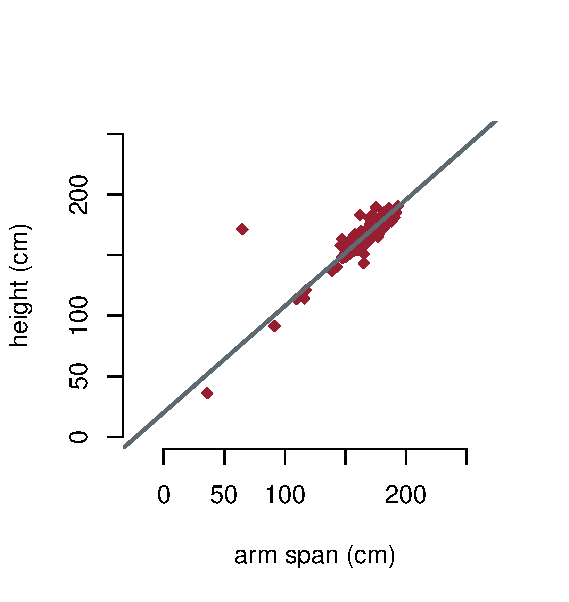
\includegraphics[trim = 0 0 0 0,clip,width=0.85\textwidth]{pdfs/OneGraphic.pdf} }
    \end{center}
    \label{fig:OneGraphic}
    \hrule
\end{figure}

Write something here.

\section{Research Question: How do body composition ratios relate to gender and age?}
\label{sec:rq}

\subsection{How many average ’head height’ lengths are males and females relative to their respective average ’height’?}
\label{sec:rq2}

\subsection{Does grouping with ratios of 'head height' and 'height' for males and females match with groupings based on age?}
\label{sec:rq3}

\subsection{How does height correspond to arm span?}
\label{sec:rq4}

\section{Data Description}
\label{sec:data}

The data has been collected for a university class project, STATS 419 at
Washington State University. Each student collected the data on oneself
and other 9 people in the best case. The measurements were
data\_collector, person\_id, side, height, head.height,
head.circumference, hand.length (left, right), hand.width (left, right),
hand.elbow (left, right), elbow.armpit (left, right), arm.reach (left,
right), arm.span, foot.length (left, right), floor.kneepit (left,
right), floor.hip (left, right), floor.navel and floor.armpit (left,
right). Additional information like units, writing, eye, eye\_color,
swinging, age, gender, quality, minutes, ethnicity and notes were also
collected. More details about the data collection process were also
identified and clarified in a handout, that each student created to give
their participants. The students had to do this at their own time. Due
to a global pandemic of Covid-19 social distancing was needed to be
followed and the data was collected by the individuals themselves with
measuring tape.

Then the professor created a large file of all the measurements together
and gave it back to us students. Now it is time to use this primary data
for data analysis. Each student had to come with research questions that
they want to study and observe. My personal research questions are: How
do body composition ratios relate to gender and age? -\textgreater{} How
many average 'head height' lengths are males and females relative to
their respective average 'height'? -\textgreater{} Does grouping with
ratios of `head height' and `height' for males and females match with
groupings based on age? -\textgreater{} How does height relate to arm
span?

For more details, reference the Appendix section.

\subsection{Summary of Sample}
\label{sec:data-sample}

The sample we found initially had a lot of noise, which required a good
clean up. The findings were some duplicate data, wrong measurements,
different notations and units and some outliers. All of these errors
have been taken into account in the clean up section. The data left is
much more less noisy and accurate to do proper Data Analysis.

\subsection{Summary Statistics of Data}
\label{sec:data-summary}

The summary statistics of the collected data includes means and standard
deviations of all variables. It also shows the quartiles and therefore
how the data is distributed. Another summary statistic can be the
dimensions of the data. The initial data set had 428 observations and 37
variables. After the instructors clean up, there were only
\ldots\ldots{} left.

\section{Key Findings}
\label{sec:findings}

The key findings from the analysis are giving the answers to my research
questions. The main research question was asking: How do body
composition ratios relate to gender and age. I only started looking at
the head height vs height proportions of every person. Then the male and
female data was separated so that I can find the average of each. The
next key finding was, that the data grouping by head height and height
proportions or height and age do give the same result for 90.25641 \% of
the time. This means, that the grouping comparisons are valid and work
well for this data. An addition to this is the interest of what
percentage is considered heroic. There I was surprised that it was 13.33
\% of the whole data when grouping based on proportions. It seemed quite
a lot to me. And out of those 13 \%, 61.53846 \% have been male. Another
grouping by internet vales of average height showed, that 53.125 \% of
categorized `heroic' people this time were male.

A very great finding was also, that height and arm span have a strong
linear relationship. The taller one person is, the wider is the
corresponding arm span. Another interesting fact about it is, that the
measurements of height and arm span of a person are almost identical.
When doing a proportion again, and then only letting values in between
0.9 and 1.1 (a 90\% match) being true, then 89.79592 of the data is
applicable.

When coming back to my primary research question, I can say, that the
body composition ratio of head height vs height do relate to gender and
more to age. It relates more to age, because a child's ratio differs
from the one of an adult. And there a clear line can be seen. Whereas,
with gender there is not much of a possible distinguish, because the
ratio of an average of 8 is the same.

\section{Conclusion}
\label{sec:conclusion}

As a conclusion I can say, that I have been able to find very
interesting results, that let me explain my research questions. I can
for sure say, that there is a lot more to learn from body composition
data.

Refer to the Appendices in section\textasciitilde{}\ref{sec:appendix}
where I am going to cite John \citep[pp. 2-3]{Tukey:1962}.

\newpage

\begin{table}[!htbp]
\footnotesize
\centering
\caption{\textbf{Descriptive Statistics and Correlation Analysis}}
\label{table:correlation}
\begin{tabularx}{0.9\textwidth}{{r@{ \ \ } p{35mm} r@{}lp{1mm} r@{}l p{5mm} r@{}l p{2mm} r@{}l p{2mm}   r@{}l  }}
 & \\
\hline
 & \\
\multicolumn{2}{c}{\textbf{ }} & \multicolumn{2}{c}{\textbf{M}} & & \multicolumn{2}{c}{\textbf{SD}} &  & \multicolumn{2}{c}{\textbf{1}} &  & \multicolumn{2}{c}{\textbf{2}} &  & \\ 
 & \\
\hline
 & \\
\textbf{1} & \textbf{Height (cm)} &  166&.9 &  &  29&.75 &  &  1&  &  &  \multicolumn{2}{c}{ \  \  \  \  \ }  &  & \\ 
 & \\
\textbf{2} & \textbf{Arm Span (cm)} &  210&.7 &  &  35&.58 &  &  &.90{$^{***}$}  &  &  1&  &  & \\ 
 & \\
\textbf{3} & \textbf{Head Height (cm)} &  22&.2 &  &  3&.56 &  &  &.66{$^{***}$}  &  &  &.66{$^{***}$}  &  & \\ 
 & \\
\hline
 & \\
\multicolumn{13}{p{0.81\textwidth}}{  \footnotesize { \begin{hangparas}{0.75in}{1} \textbf{\underline{Notes}:} \ \ Pearson pairwise correlations are reported; \newline a two-side test was performed to report correlation significance.  \end{hangparas} } }  & \\  
\multicolumn{13}{p{0.81\textwidth}}{  {\tiny {$^{\dagger} p < .10$} }  {     } {\tiny        {$^{*} p < .05$} }  {     } {\tiny       {$^{**} p < .01$} }  {     } {\tiny      {$^{***} p < .001$} } {     }     } & \\ 
 & \\
\hline
\end{tabularx}
\end{table}


\newpage

\newpage
\section{APPENDICES}
\label{sec:appendix}

\subsection{Data Provenance}
\label{sec:appendix-data-provenance}

Data Provenance is very crucial and important in this project and for
every data collection process and data analytics evaluation. The data
collection is one of the most important steps in data analytics, it
requires authenticity, enabling trust into the data and allowing
reproducibility. The origin of the data are students in a university
statistics class, that took the body measurements themselves. All of the
data then was combined into one text file by the instructor. The
validation of the initial data turns out to be not as trust worthy as
expected. There have been evaluated some duplicate and wrong data which
have been cleaned up in a self clean up process and also by the
instructor, who later on provided a cleaned data set in order to be sure
of data provenance and having data to trust.

The data is reproducible. To reproduce the data a handout has been
created. It is attached below for reference.

\newpage
\subsubsection{Data Collection Handout}
\label{sec:appendix-data-handout}

\begin{figure}[!ht]
    \hrule
    \caption{ \textbf{Handout Page 1} }
    \begin{center}
        \scalebox{1.00}{    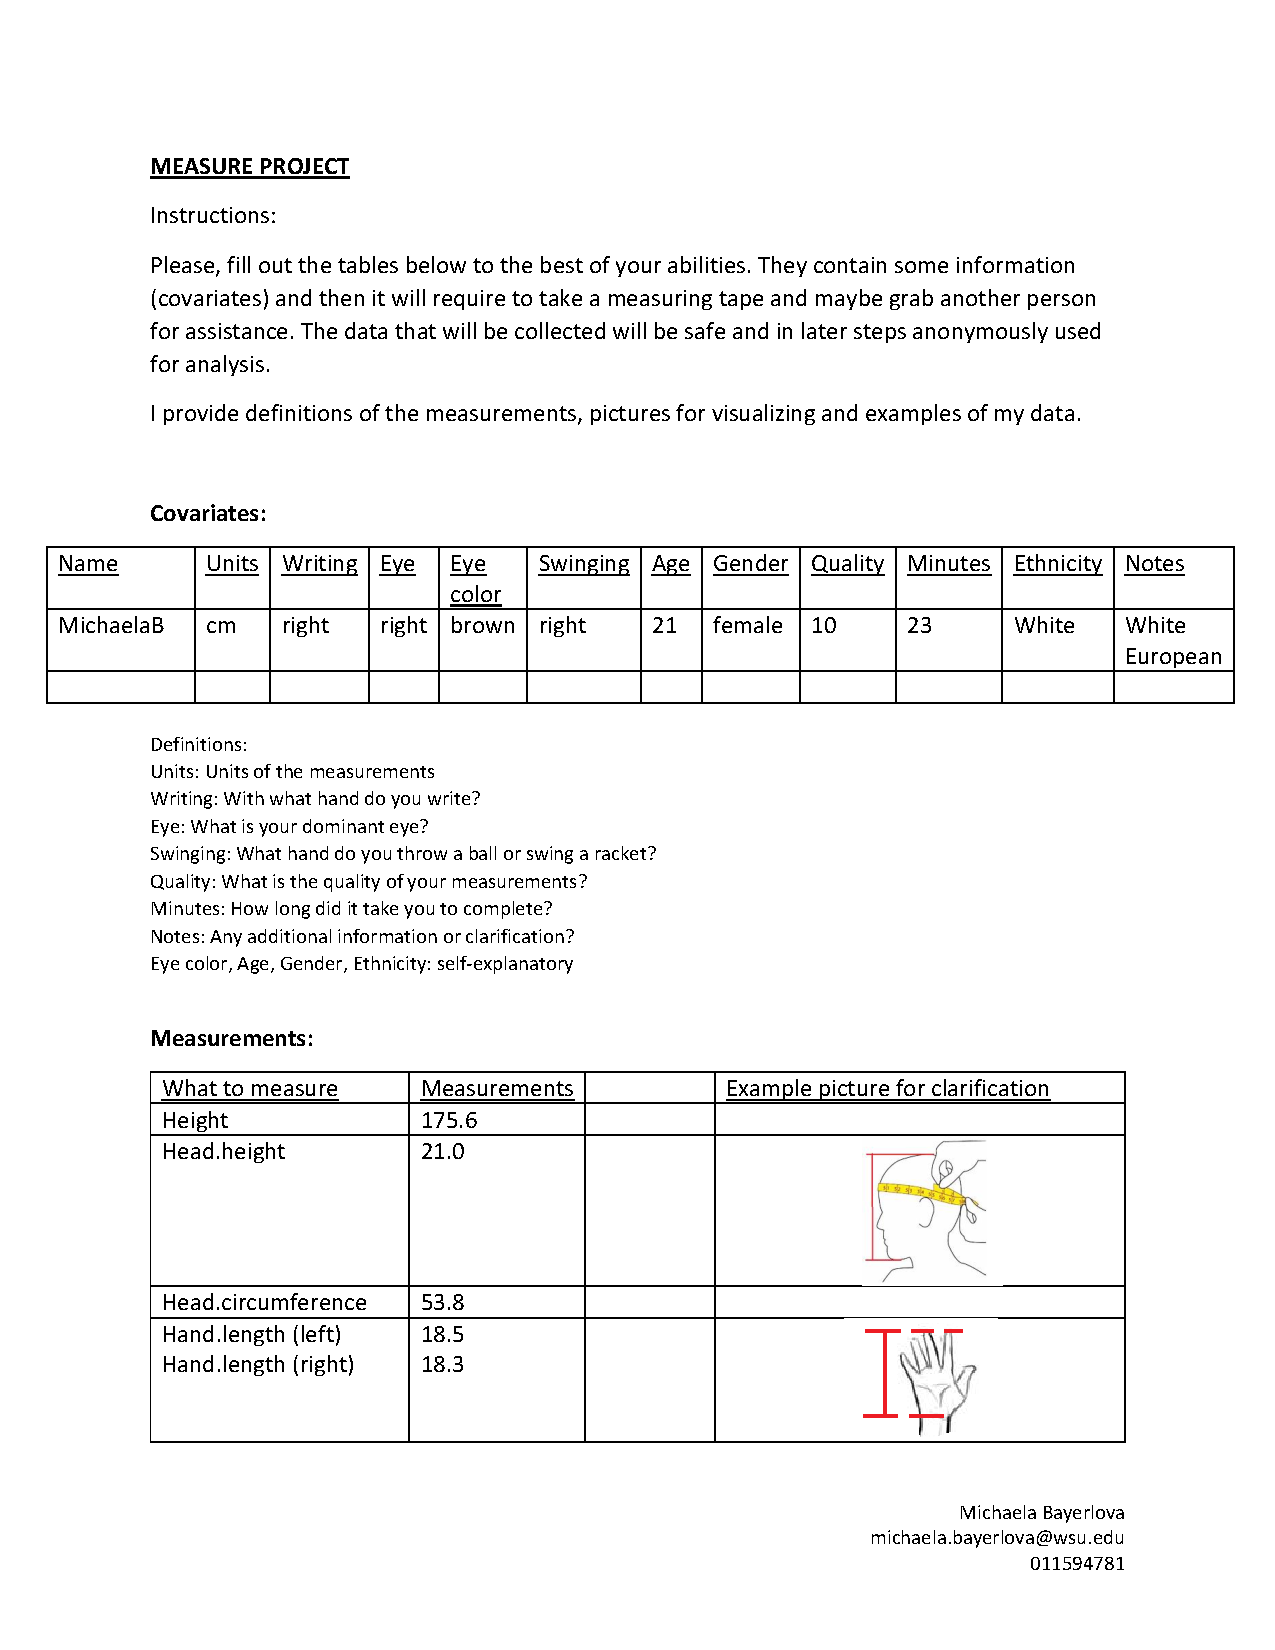
\includegraphics[trim = 0 0 0 0,clip,width=0.85\textwidth]{pdfs/2.Handout_page1.pdf} }
    \end{center}
    \label{fig:handout-1}
    \hrule
\end{figure}

\newpage

\begin{figure}[!ht]
    \hrule
    \caption{ \textbf{Handout Page 2} }
    \begin{center}
        \scalebox{1.00}{    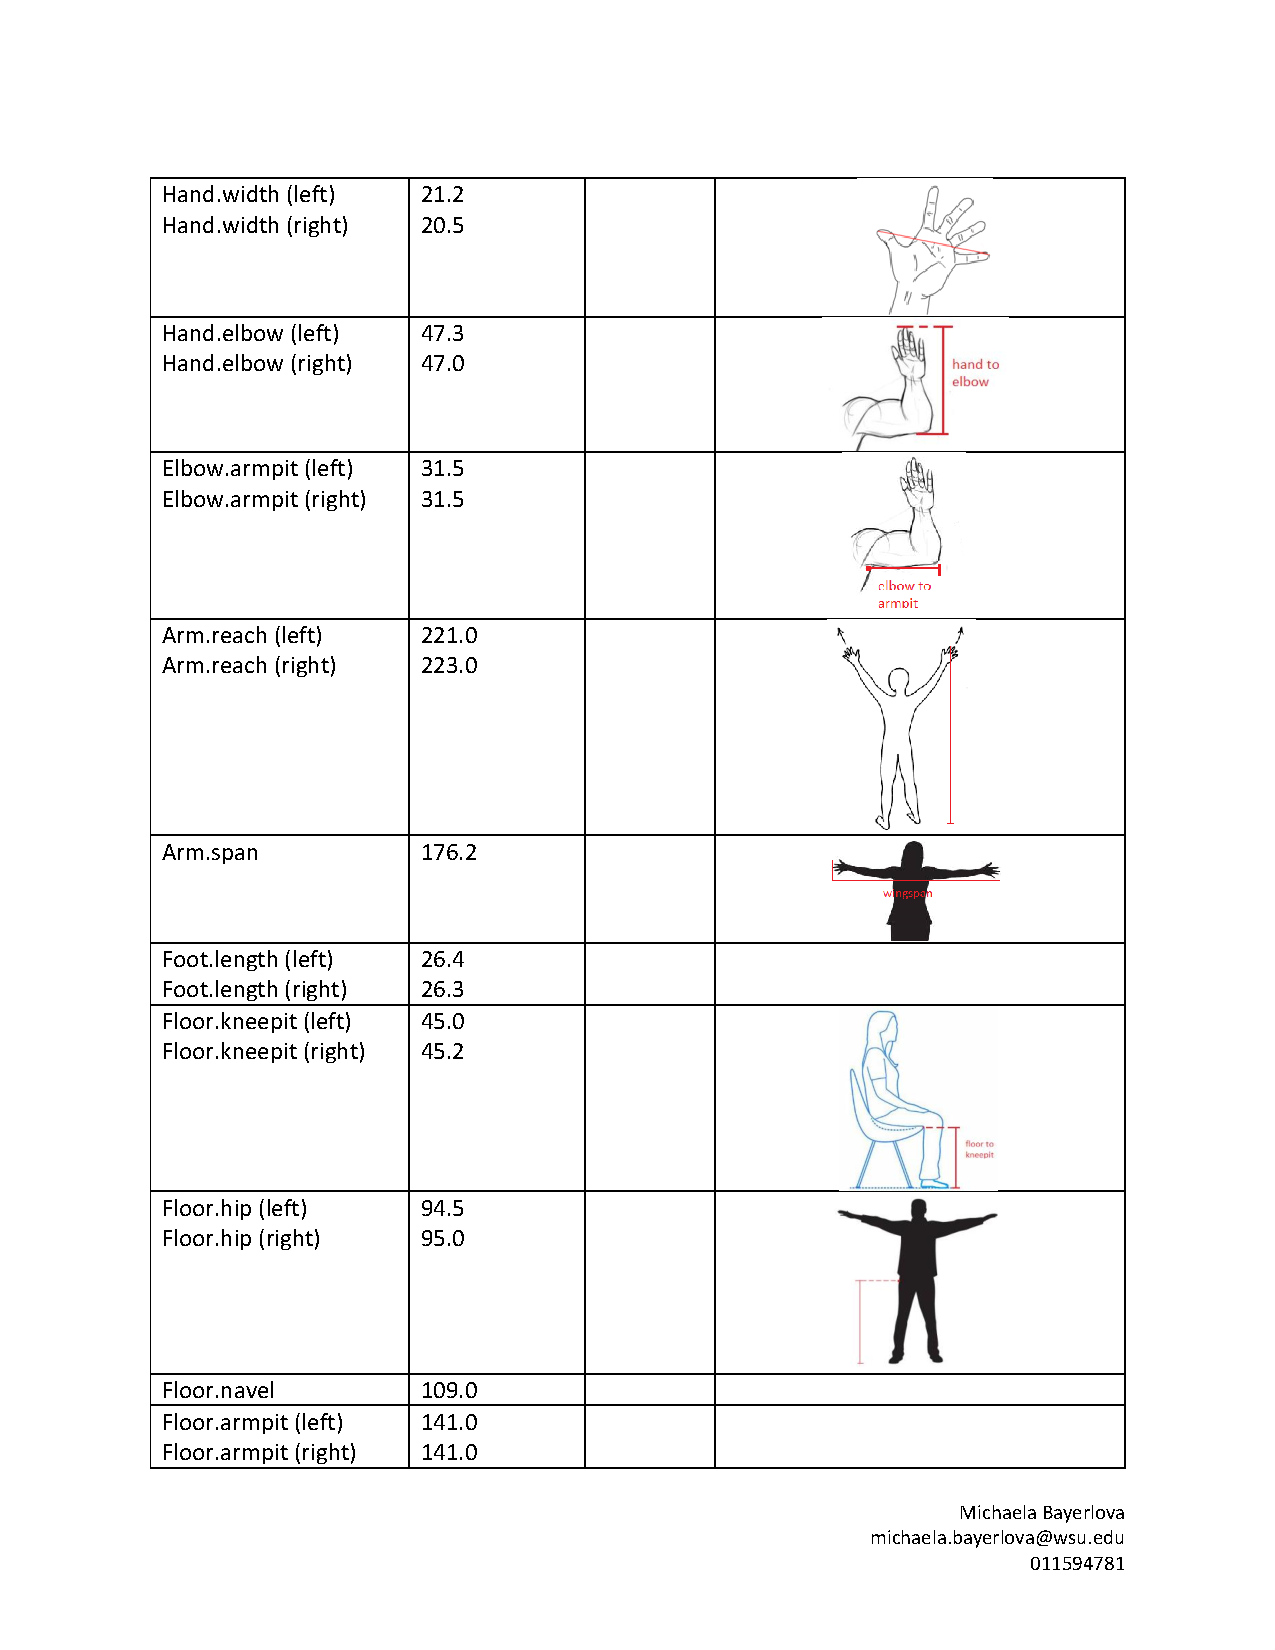
\includegraphics[trim = 0 0 0 0,clip,width=0.85\textwidth]{pdfs/2.Handout_page2.pdf} }
    \end{center}
    \label{fig:handout-2}
    \hrule
\end{figure}

\newpage

\begin{figure}[!ht]
    \begin{subfigure}[h]{0.5\textwidth}
    \centering
    %  trim={<left> <lower> <right> <upper>}
    % https://shantoroy.com/latex/add-subfig-in-latex/
            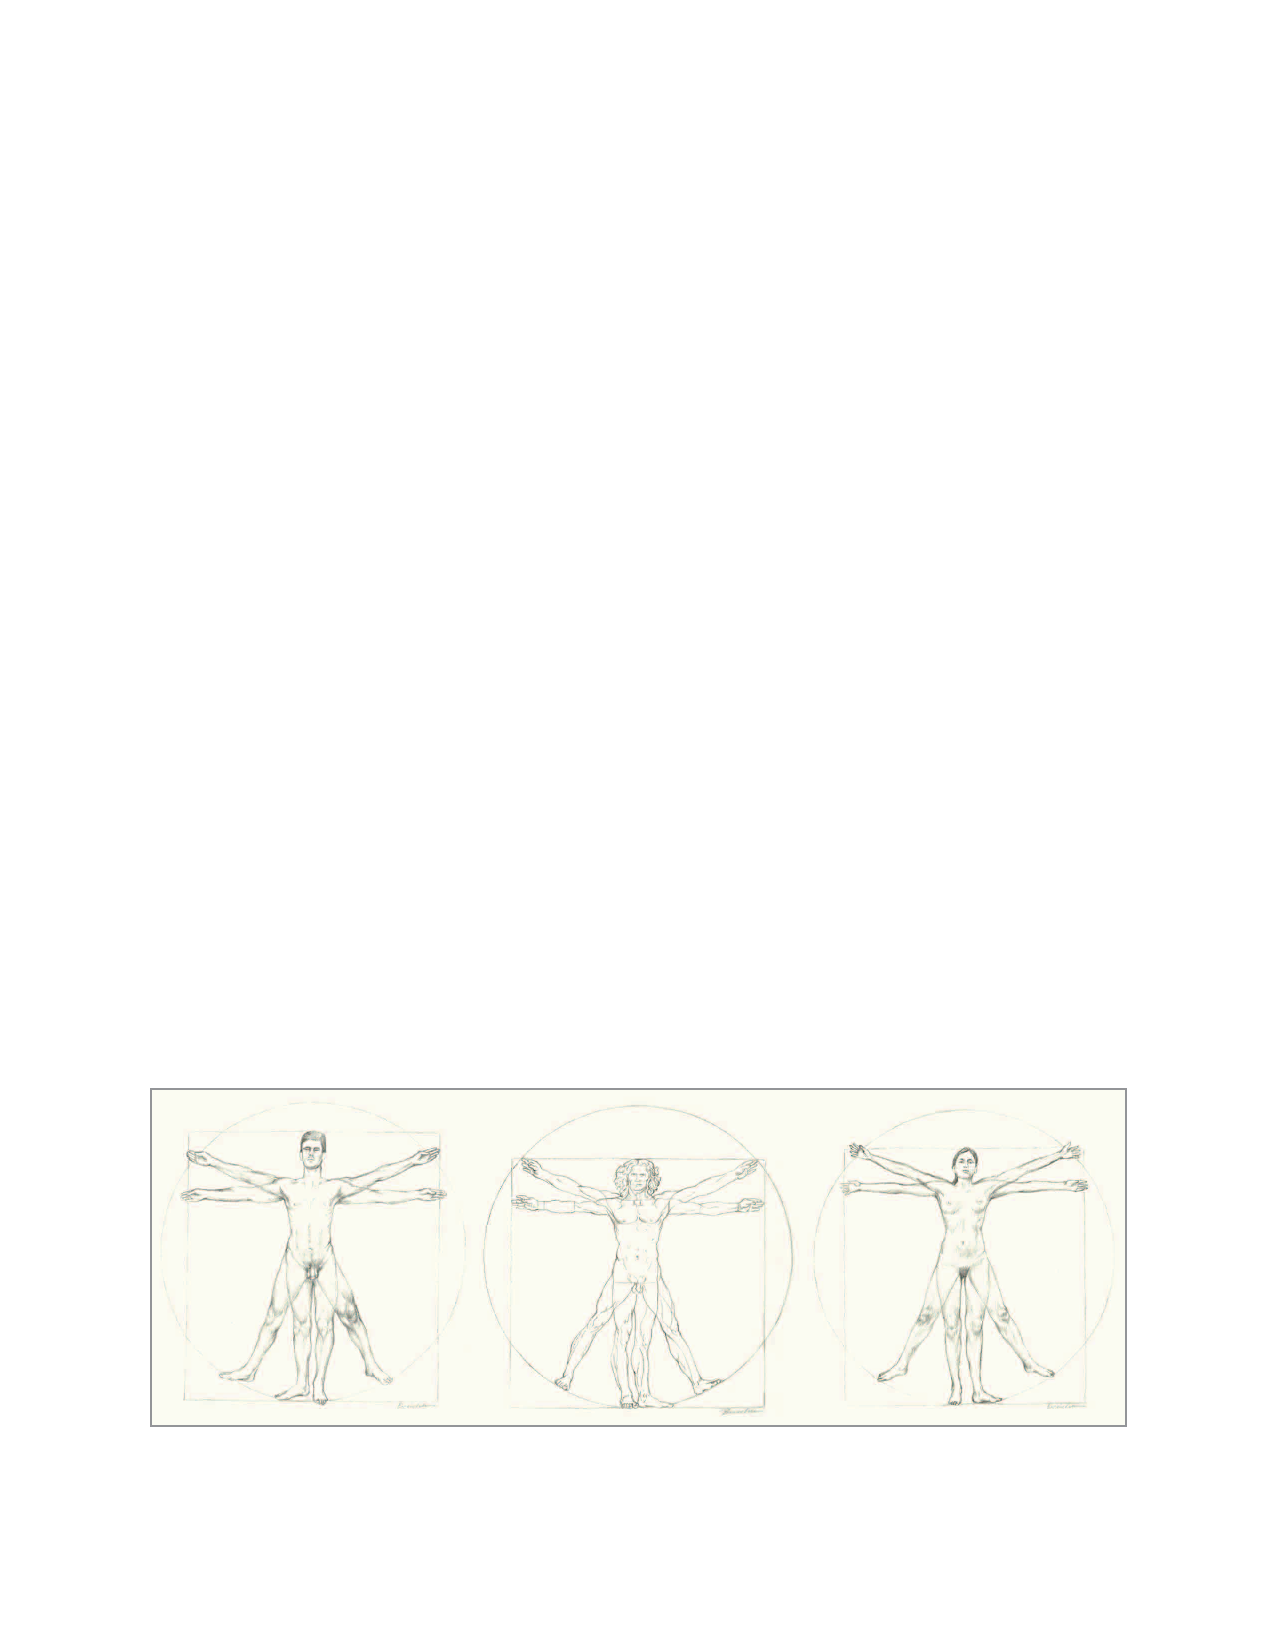
\includegraphics[trim = 0 0 11.25cm 0,clip,scale=1]{figures/Vitruvian.pdf}
        \caption{ \citet{Thomas:2020} discuss this. }
        \label{fig:sub-first}
    \end{subfigure}
    \begin{subfigure}[h]{0.5\textwidth}
    \centering
        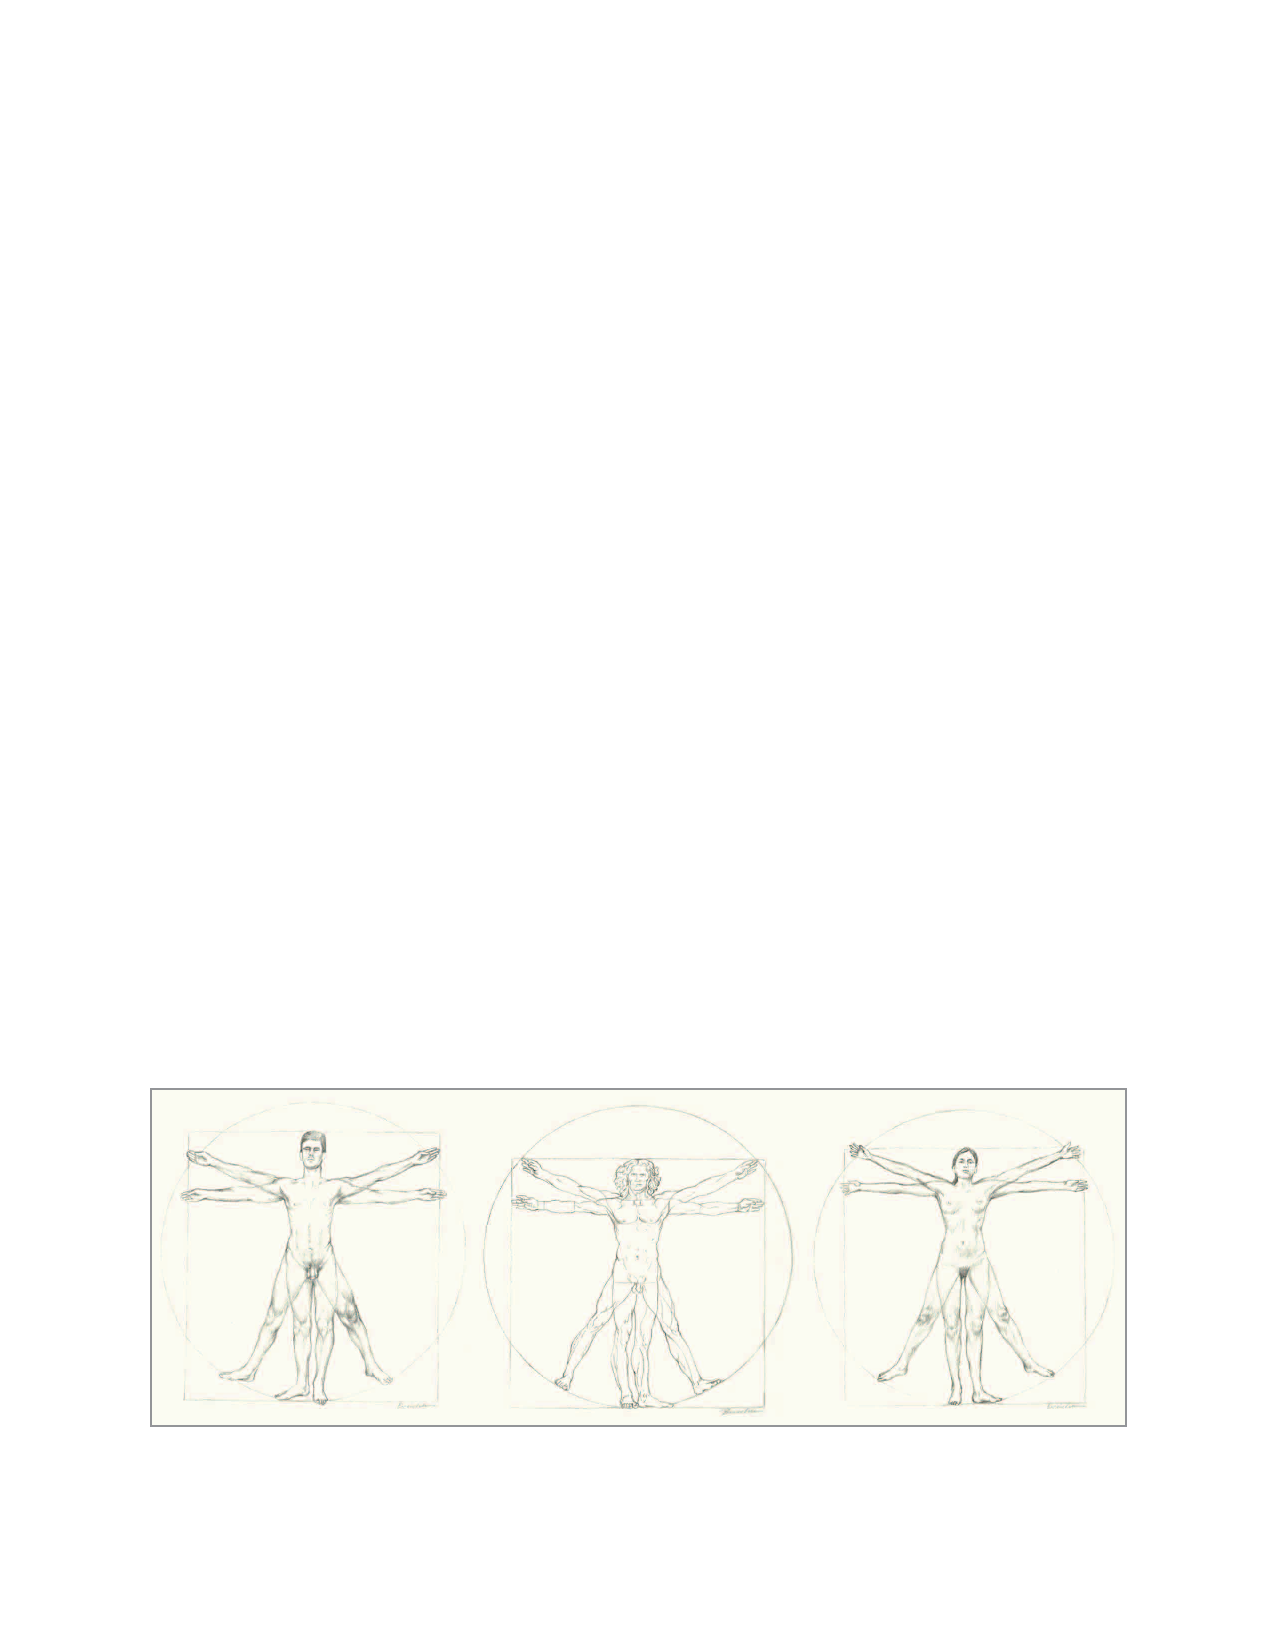
\includegraphics[trim = 11.25cm 0 0 0,clip,scale=1]{figures/Vitruvian.pdf}
            \caption{Schnitt realer Sensor \citep{Thomas:2020}}
        \label{fig:sub-second}
    \end{subfigure}
    \vspace{2.5mm}
    \hrule
    \vspace{2.5mm}
        \caption{\textbf{ Der Sensor in Theorie und Verwirklichung.}   }
        \label{fig:combined}
    \vspace{-2.5mm}
    \hrule
\end{figure}

\newpage

\subsection{Preparing the Report Workspace}
\label{sec:appendix-prepare-workspace}

Below is the necessary functions and libraries required to run the code
referenced in this document.

\begin{Shaded}
\begin{Highlighting}[]
\KeywordTok{library}\NormalTok{(devtools);       }\CommentTok{\# required for source\_url}

\NormalTok{path.humanVerseWSU =}\StringTok{ "https://raw.githubusercontent.com/MonteShaffer/humanVerseWSU/"}
\KeywordTok{source\_url}\NormalTok{( }\KeywordTok{paste0}\NormalTok{(path.humanVerseWSU,}\StringTok{"master/misc/functions{-}project{-}measure.R"}\NormalTok{) );}

\NormalTok{path.functions =}\StringTok{ ""}
\end{Highlighting}
\end{Shaded}

Below is the code to load the data and prepare it for analysis.

\begin{Shaded}
\begin{Highlighting}[]
\NormalTok{path.project =}\StringTok{ "C:/Users/michaela.bayerlova/Documents/STATS 419/measurement\_project/michaela/project{-}measure/"}\NormalTok{;}

\NormalTok{path.to.secret =}\StringTok{ "C:/\_git\_/SECRETS/"}\NormalTok{;}

\NormalTok{file.measure =}\StringTok{ }\KeywordTok{paste0}\NormalTok{(path.to.secret,}\StringTok{"measure{-}students.txt"}\NormalTok{);}
\NormalTok{file.measure.clean =}\StringTok{ }\KeywordTok{paste0}\NormalTok{(path.to.secret,}\StringTok{"cm.final.measure.txt"}\NormalTok{);}

\NormalTok{path.github =}\StringTok{ "https://raw.githubusercontent.com/MichaelaB1/WSU\_STATS419\_FALL2020/"}\NormalTok{;}
\KeywordTok{source\_url}\NormalTok{( }\KeywordTok{paste0}\NormalTok{(path.github,}\StringTok{"master/Project1/michaela\_project\_measure/functions/functions\_project\_measure.R"}\NormalTok{) );}

\CommentTok{\# this is your function}
\CommentTok{\# put in the same "units"}
\CommentTok{\# merge left/right}
\CommentTok{\# build proportion data}
\CommentTok{\# and so on ... }
\CommentTok{\# measure.df = prepareMeasureData(measure);}
\end{Highlighting}
\end{Shaded}

\newpage

\subsection{Self Data Cleanup}
\label{sec:appendix-self-data-cleanup}

\paragraph{Create data frame measure}
\label{sec:appendix-create-data-frame-measure}

At first the data is read into the program and then I save the original
data in a data frame called measure.raw. Another data frame is created
as well, measure.clean, which is going to be modified and cleaned. To
get an initial basic idea and overview about the data, I view the
dimensions and summary statistics of the data set.

\paragraph{Remove Duplicates}
\label{sec:appendix-remove-duplicates}

As the next step, the duplicates function is given to use by the
instructor to use.

\paragraph{Average values}
\label{sec:appendix-average-values}

The initial collected data has some entries that have one measurement
like height, but then there are also measurements of left and right
side, for example the hand length. For data points that have a right and
left measurements, the average will be taken in this function. When
there is only one measurement, that one will be taken. This enables to
get a uniform set of data without missing values for those entries.
These new average values are added in new columns to the end of the data
frame.

\paragraph{Leave only average values}
\label{sec:appendix-leave-avg-values}

This section is cleaning up the data frame from above. The single
entries of average values will be placed instead of the left and right
data, which are removed. For further analysis the `notes' column is not
needed and is therefore removed as well.

\paragraph{Unity among gender notation}
\label{sec:appendix-gender-notation}

In the collected data, there have been used different notations to
indicate `female' and `male'. This will cause problems in further
analyses and it therefore needs to be adjusted to an overall standard.
The standard will be the one provided above. First of all, the whole
string entries in the column `gender' will be converted to lower case
characters. Then the wrong assigned data will be newly assigned to
`female' or `male'.

\paragraph{Converting units to cm}
\label{sec:appendix-convert-units-cm}

Since not all data has been collected in the same units, this has to be
fixed in order to compare the data properly. Units used are inches and
cm. I have decided to go with cm, so I convert inches to cm, where 1
inch equals to 2.54 cm. Before applying the math there, I have to also
change the notation of units of inches. There have been used `inches',
`Inch', `in' and `inch'. The last notation is the preferred one to use.
After this change has been made, the unit conversion takes place.

\paragraph{Remove wrong data}
\label{sec:appendix-wrong-data}

This step is removing data that cannot be true. For example observations
of the data showed, that some arm.reach data point are smaller than the
normal height. This cannot be true, it is a wrong measurement and needs
to be removed. So the code compares these 2 columns, when a comparison
is false the entry will be removed from the data frame.

\paragraph{Remove Outliers}
\label{sec:appendix-remove-outliers}

This step enables to clean up the data even more such that it has only
accurate and reasonable data. The method used uses quantiles and IQR.
The data has to be free of NA values first.

\subparagraph{Findings: Clean up}
\label{sec:appendix-findings-clean-up}

The clean up removed the main noisy and wrong data, so that the further
analysis is taken upon good data to trust and also to trust the analysis
results.

Below is the self data clean up function that has all the steps inside
of them.

\begin{Shaded}
\begin{Highlighting}[]
\NormalTok{measure.clean =}\StringTok{ }\KeywordTok{prepareMeasureData}\NormalTok{(file.measure);}
\end{Highlighting}
\end{Shaded}

\newpage

\subsection{Instructor Data Cleanup}
\label{sec:appendix-instructor-data-cleanup}

The instructor has provided another cleaned data set to the students
after some issues have arised.

Therefore, only a new text file needs to be loaded and read in as a data
frame.

\begin{Shaded}
\begin{Highlighting}[]
\NormalTok{measure.clean2 =}\StringTok{ }\KeywordTok{readDataIntoDataFrame}\NormalTok{(file.measure.clean);}
\end{Highlighting}
\end{Shaded}

\newpage

\subsection{Data Analysis}
\label{sec:appendix-data-analysis}

\subsubsection{Proportions of head.height vs whole body height}
\label{sec:appendix-height-vs-head.height}

\paragraph{Create a subset with only important variables for the analysis}
\label{sec:appendix-create-subset}

This step creates a subset of the data, so that only the variables are
taken which are needed and used for analysis later. This step can be
done even without cleaning up the data before from NA values, this way
the rows with empty values in other columns do not affect the data
subset here, because it still can be used. And the missing values only
in these columns can be removed later. The columns left are `height.NA',
`head.height.NA', `arm.span.NA', `age' and `gender'. The others are
dropped.

\paragraph{Create new data frame 'measure.proportions' to work on analysis}
\label{sec:appendix-create-data-frame-no-NA}

Right now the NA values from the subset data frame are removed with the
na.omit() command.

\paragraph{Assign proportions group}
\label{sec:appendix-assign-proportions-group}

This analysis is based on the calculation of how many times the head
height fits into the whole body height. Then the proportion values will
be grouped into different groups, these are: Group `F': There the person
is most likely a female adult because the proportions are bigger than
what kids usually have, which is above 6.5. Group `M': There the person
is most likely a male adult because the proportions are bigger than what
kids usually have, which is above 6.5. Group `K': There the person is
most likely a child (male or female) because the proportions are smaller
or equal to 6.5.

\paragraph{Assign age group}
\label{sec:appendix-assign-age-group}

This analysis is based on the age and gender of a person. Then these
groups are created: Group `F': There the person is female and 11 years
or older. Group `M': There the person is male and 11 years or older.
Group `K': There the person is a child (male or female) because the age
is 10 or younger.

\subparagraph{Findings: Assigning proportions and age group}
\label{sec:appendix-findings-assign-age-group}

The results give three new columns in the data frame. One where the
proportions of height/head.height are given, another where these
proportions are used to assign each to a label (`F', `M' or `K'). These
same labels are also assigned in the third column, where the criterion
is age. This gained information will then especially be used to compare
the 2 assignment methods.

The code for this step is showed below.

\begin{Shaded}
\begin{Highlighting}[]
\CommentTok{\# Prepare for analysis of proportions}
\NormalTok{measure.proportions =}\StringTok{ }\KeywordTok{prepareProportionsAnalysis}\NormalTok{(measure.clean);}

\CommentTok{\# same step for instructors data}
\NormalTok{measure.proportions2 =}\StringTok{ }\KeywordTok{prepareProportionsAnalysis}\NormalTok{(measure.clean2);}
\end{Highlighting}
\end{Shaded}

\newpage

\subsubsection{What is the mean of male or female proportions?}
\label{sec:appendix-mean-gender-proportions}

Here the newly created proportions of male and female get separated into
new data frames, so that the mean and other statistical values of each
can be viewed with the summary() command.

\paragraph{Findings: Mean of male and female proportions}
\label{sec:appendix-findings-mean-gender-proportions}

The findings are, that the mean proportions of head heights in the
height of females in the data set is about \ldots. The mean value I get
for males is \ldots{}

Below is the code for the summary statistics of male and female head
height vs height proportions.

\begin{Shaded}
\begin{Highlighting}[]
\CommentTok{\# Summary statistics of male and female proportions}
\KeywordTok{meanGenderProportions}\NormalTok{(measure.proportions);}
\end{Highlighting}
\end{Shaded}

\begin{verbatim}
##    height.NA     head.height.NA   arm.span.NA         age       
##  Min.   : 27.3   Min.   : 6.50   Min.   : 36.0   Min.   : 3.00  
##  1st Qu.:156.6   1st Qu.:20.05   1st Qu.:154.9   1st Qu.:21.50  
##  Median :162.5   Median :21.00   Median :163.0   Median :28.00  
##  Mean   :157.5   Mean   :21.36   Mean   :159.6   Mean   :34.99  
##  3rd Qu.:167.7   3rd Qu.:22.68   3rd Qu.:171.0   3rd Qu.:52.00  
##  Max.   :181.0   Max.   :33.02   Max.   :185.5   Max.   :94.00  
##     gender          proportions.head.and.height proportions.group 
##  Length:99          Min.   :1.344               Length:99         
##  Class :character   1st Qu.:6.992               Class :character  
##  Mode  :character   Median :7.563               Mode  :character  
##                     Mean   :7.431                                 
##                     3rd Qu.:8.131                                 
##                     Max.   :9.278                                 
##   age.group        
##  Length:99         
##  Class :character  
##  Mode  :character  
##                    
##                    
## 
\end{verbatim}

\begin{Shaded}
\begin{Highlighting}[]
\CommentTok{\# same step for instructors data}
\KeywordTok{meanGenderProportions}\NormalTok{(measure.proportions2);}
\end{Highlighting}
\end{Shaded}

\begin{verbatim}
##   head.height  head.circumference   swinging           arm.reach  
##  Min.   : NA   Min.   : NA        Length:0           Min.   : NA  
##  1st Qu.: NA   1st Qu.: NA        Class :character   1st Qu.: NA  
##  Median : NA   Median : NA        Mode  :character   Median : NA  
##  Mean   :NaN   Mean   :NaN                           Mean   :NaN  
##  3rd Qu.: NA   3rd Qu.: NA                           3rd Qu.: NA  
##  Max.   : NA   Max.   : NA                           Max.   : NA  
##   foot.length    my.units         my.ethnicity        my.gender        
##  Min.   : NA   Length:0           Length:0           Length:0          
##  1st Qu.: NA   Class :character   Class :character   Class :character  
##  Median : NA   Mode  :character   Mode  :character   Mode  :character  
##  Mean   :NaN                                                           
##  3rd Qu.: NA                                                           
##  Max.   : NA                                                           
##   new.units            my.eye           my.writing        my.swinging       
##  Length:0           Length:0           Length:0           Length:0          
##  Class :character   Class :character   Class :character   Class :character  
##  Mode  :character   Mode  :character   Mode  :character   Mode  :character  
##                                                                             
##                                                                             
##                                                                             
##  my.eye.color       proportions.head.and.height proportions.group 
##  Length:0           Min.   : NA                 Length:0          
##  Class :character   1st Qu.: NA                 Class :character  
##  Mode  :character   Median : NA                 Mode  :character  
##                     Mean   :NaN                                   
##                     3rd Qu.: NA                                   
##                     Max.   : NA                                   
##   age.group        
##  Length:0          
##  Class :character  
##  Mode  :character  
##                    
##                    
## 
\end{verbatim}

\newpage

\subsubsection{Do group age and proportions match?}
\label{sec:appendix-group-age-vs-proportions}

\paragraph{Create data frame with newly created 3 columns}
\label{sec:appendix-new-proportions-df}

A new data frame will be created now with only the newly created
columns.

\paragraph{Comparison age vs proportions group}
\label{sec:appendix-comparison-age-vs-proportions-group}

Here the analysis gets interesting. Now we compare if the two ways of
assigning groups are matching in the assigned groups. The one way is
assigning it by proportions of height/head.height and gender, the other
way by age and gender. The result is a percentage of how many assigned
labels match.

\subparagraph{Findings: Comparison age vs proportions group}
\label{sec:appendix-findings-comparison-age-vs-proportions-group}

The results give a percentage of about 90.26 \%. This means that 9 out
of 10 assignments using method 1 to assign by proportions and the method
2 to assign by age will give the same result.

Below the code for the comparison of group age and group proportions is
shown.

\begin{Shaded}
\begin{Highlighting}[]
\CommentTok{\# \# Do the 2 groups assigned match}
\CommentTok{\# match.percentage = matchingGroups(measure.proportions);}
\CommentTok{\# }
\CommentTok{\# \# same step for instructors data}
\CommentTok{\# match.percentage2 = matchingGroups(measure.proportions2);}
\end{Highlighting}
\end{Shaded}

\newpage

\paragraph{What percentage of people is considered 'heroic'?}
\label{sec:appendix-heroic}

\subparagraph{Assign heroic based on head.height vs height proportions}
\label{sec:appendix-heroic-proportions}

This analysis is based on the calculation of how many times the head
height fits into the whole body height. Then the proportion values will
be grouped into different groups, these are: Group `F': There the person
is most likely a female adult because the proportions are bigger than
what kids usually have, which is above 6.5 and below or equal to 8.5.
Group `M': There the person is most likely a male adult because the
proportions are bigger than what kids usually have, which is above 6.5
and below or equal to 8.5. Group `K': There the person is most likely a
child (male or female) because the proportions are smaller or equal to
6.5. Group `H': There the person is most likely an adult because the
proportions are heroic above 8.5. The result is a percentage of how many
assignments from the data are `heroic'.

\subparagraph{Findings: Heroic}
\label{sec:appendix-findings-heroic}

The results give a percentage of about 13.3 \%. This means that 13 out
of every 100 people is considered heroic, and therefore taller than the
average height when looking at the head.height vs height proportions
only!

Below the code for the comparison of group age and group proportions is
shown.

\begin{Shaded}
\begin{Highlighting}[]
\CommentTok{\# \# What percentage of people is considered heroic?}
\CommentTok{\# h.percentage = heroicPeople(measure.proportions);}
\CommentTok{\# }
\CommentTok{\# \# same step for instructors data}
\CommentTok{\# h.percentage2 = heroicPeople(measure.proportions2);}
\end{Highlighting}
\end{Shaded}

\newpage

\paragraph{What percentage is male out of assigned heroic people?}
\label{sec:appendix-heroic-proportions-percentage}

From the assigned percentage of heroic people over the total
assignments, now the percentage of that assigned heroic people that are
male will be found out with a function. And the assignments left have to
be the female ones.

\subparagraph{Findings: Heroic male percentage}
\label{sec:appendix-findings-heroic-male-percentage}

The results give a percentage of the people that are male out of the
assigned heroic people. This is found to be 61.53846 \% (male out of
heroic).

Below the code of percentages of heroic males and heroic females are
given.

\begin{Shaded}
\begin{Highlighting}[]
\CommentTok{\# \# What percentage of heroic people are male}
\CommentTok{\# heroic.male.p = percentageOfHeroicPeopleBeingMale(measure.proportions);}
\CommentTok{\# heroic.female.p = 100 {-} heroic.male.p;}
\CommentTok{\# }
\CommentTok{\# \# same for instructors data}
\CommentTok{\# heroic.male.p2 = percentageOfHeroicPeopleBeingMale(measure.proportions2);}
\CommentTok{\# heroic.female.p2 = 100 {-} heroic.male.p2;}
\end{Highlighting}
\end{Shaded}

\newpage

\paragraph{Assign heroic based on height}
\label{sec:appendix-heroic-height}

Here a major part is the reference to a website
``\url{https://ourworldindata.org/human-height}'' where the comparison
data for the assignment was taken from. There is says that the average
height for male around the world is 171 cm and for female 159 cm. So
every height in our data that is higher will be considered as heroic.
Also specified is the gender to get a percentage of how many heroic male
there are compared to female.

\subparagraph{Findings: Heroic Height}
\label{sec:appendix-findings-heroic-height}

The results give a percentage of the people that are male out of the
assigned heroic people. That percentage is 53.125.

Below the code of percentages of heroic males and heroic females are
given.

\begin{Shaded}
\begin{Highlighting}[]
\CommentTok{\# \# Assign people heroic based on height and get percentage}
\CommentTok{\# heroic.m.p = assignHeroicByHeightMalePercentage(measure.proportions);}
\CommentTok{\# heroic.f.p = 100 {-} heroic.m.p;}
\CommentTok{\# }
\CommentTok{\# \# same for instructors data}
\CommentTok{\# heroic.m.p2 = assignHeroicByHeightMalePercentage(measure.proportions2);}
\CommentTok{\# heroic.f.p2 = 100 {-} heroic.m.p2;}
\end{Highlighting}
\end{Shaded}

\newpage

\subsubsection{How does arm span relate to height?}
\label{sec:appendix-arm-span-vs-height}

Another research question's interest is the relationship between
arm.span and height.

\paragraph{Plotting variables}
\label{sec:appendix-plotting-variables}

This is a really interesting analysis. Since we know from the Figure 4.
that a person should have around the same height and arm span it should
be also verified in this sections analysis. A human proportions are
given like this.

\subparagraph{Findings of plotting variables}
\label{sec:appendix-findings-plotting}

When making a plot and viewing a summary statistics the plot we see is a
linear line graph. It clearly shows a linear relationship between those
two variables. The axis labels are also the same, which means that it is
nearly a slope of 1, which would be perfectly linear. The summary
statistics also proves that because the mean, 1st and 3rd Quartile
values are very close.

\begin{Shaded}
\begin{Highlighting}[]
\CommentTok{\# \# Is there a linear relationship between the two variables? {-}\textgreater{} Yes}
\CommentTok{\# plot(measure.proportions$arm.span.NA, measure.proportions$height.NA, col = "blue",main = paste("Plot of arm.span vs height of measure.proportions data"), xlab = paste("arm.span.NA (cm)"), ylab = paste("height.NA (cm)"));}
\CommentTok{\# summary(measure.proportions);}
\CommentTok{\# }
\CommentTok{\# \# same step for instructors data}
\CommentTok{\# plot(measure.proportions2$arm.span.NA, measure.proportions2$height.NA, col = "darkblue",main = paste("Plot of arm.span vs height of measure.proportions2 data"), xlab = paste("arm.span.NA (cm)"), ylab = paste("height.NA (cm)"));}
\CommentTok{\# summary(measure.proportions2);}
\end{Highlighting}
\end{Shaded}

Below is the code for the comparison of a 90\% match.

\begin{Shaded}
\begin{Highlighting}[]
\CommentTok{\# \# Is there a relationship between arm.span and height?}
\CommentTok{\# match.percentage.90 = relateArmSpanAndHeight(measure.proportions);}
\CommentTok{\# }
\CommentTok{\# \# same step for instructors data}
\CommentTok{\# match.percentage.90.2 = relateArmSpanAndHeight(measure.proportions2);}
\end{Highlighting}
\end{Shaded}

\newpage

\subsubsection{Proportions of all measurements vs head.height}
\label{sec:appendix-proportions}

This is of additional interest for additional observations.

Below the code for the comparison of group age and group proportions is
shown.

\begin{Shaded}
\begin{Highlighting}[]
\CommentTok{\# \# Proportions of all measurements vs head.height}
\CommentTok{\# measure.head.proportions = proportionsAllColumnsVSHeadHeight(measure.clean);}
\CommentTok{\# }
\CommentTok{\# \# same step for instructors data}
\CommentTok{\# measure.head.proportions2 = proportionsAllColumnsVSHeadHeight(measure.clean2);}
\end{Highlighting}
\end{Shaded}

\newpage

\subsubsection{Statistical analysis}
\label{sec:appendix-statistical-analysis}

\paragraph{Correlation and t-test}
\label{sec:appendix-correlation-and-ttest}

This section includes a correlation test and t-test upon some variables
of the data. Those variables are the main variables of interest. Each
correlation and t-test is done on 2 variables only.

\subparagraph{Findings: Correlation and t-test}
\label{sec:appendix-findings-correlation-and-ttest}

My data: The correlation test between height and head height gives a
correlation score of 0.6565967 with a really small p-value. Therefore,
these 2 variables have a quite strong correlation. When looking at
height and age, I would expect only a small correlation, because kids
that are young are not grown up and relatively short. When grown up the
difference of height is high and usually when getting really old then
the height does not increase anymore, it rather decreases. So that is
not a linear relationship at all. This is true, because the correlation
score is only 0.05830303 at a p-value of 0.417. Whereas height and arm
span do have a strong correlation again. The height does almost exactly
match the arm span. Therefore the score is 0.8785036 and the p-value
again very small, telling the correlation is strong. When looking at the
t-test, then we see again, that the variables height and head height,
height and age are different from each other when looking at the sample
means, whereas the height and arm span do not differ much. Then have
almost the same sample means and a high p-value instead.

Below the code for the correlation test and t-test is shown.

\begin{Shaded}
\begin{Highlighting}[]
\CommentTok{\# \# correlation}
\CommentTok{\# cor.test(measure.proportions$height.NA, measure.proportions$head.height.NA);}
\CommentTok{\# cor.test(measure.proportions$height.NA, measure.proportions$age);}
\CommentTok{\# cor.test(measure.proportions$height.NA, measure.proportions$arm.span.NA);}
\CommentTok{\# }
\CommentTok{\# \# same for instructor data}
\CommentTok{\# cor.test(measure.proportions2$height.NA, measure.proportions2$head.height.NA);}
\CommentTok{\# cor.test(measure.proportions2$height.NA, measure.proportions2$age);}
\CommentTok{\# cor.test(measure.proportions2$height.NA, measure.proportions2$arm.span.NA);}
\CommentTok{\# }
\CommentTok{\# }
\CommentTok{\# \# T{-}test}
\CommentTok{\# t.test(measure.proportions$height.NA, measure.proportions$head.height.NA);}
\CommentTok{\# t.test(measure.proportions$height.NA, measure.proportions$age);}
\CommentTok{\# t.test(measure.proportions$height.NA, measure.proportions$arm.span.NA);}
\CommentTok{\# }
\CommentTok{\# \# same for instructor data}
\CommentTok{\# t.test(measure.proportions2$height.NA, measure.proportions2$head.height.NA);}
\CommentTok{\# t.test(measure.proportions2$height.NA, measure.proportions2$age);}
\CommentTok{\# t.test(measure.proportions2$height.NA, measure.proportions2$arm.span.NA);}
\end{Highlighting}
\end{Shaded}

\paragraph{Correlation table}
\label{sec:appendix-correlation-table}

Below is the code to generate the correlation table that you see in
Section \ref{sec:conclusion}.

\begin{Shaded}
\begin{Highlighting}[]
\KeywordTok{library}\NormalTok{(devtools);       }\CommentTok{\# required for source\_url}
\NormalTok{path.humanVerseWSU =}\StringTok{ "https://raw.githubusercontent.com/MonteShaffer/humanVerseWSU/"}
\KeywordTok{source\_url}\NormalTok{( }\KeywordTok{paste0}\NormalTok{(path.humanVerseWSU,}\StringTok{"master/misc/functions{-}project{-}measure.R"}\NormalTok{) );}
\NormalTok{path.project =}\StringTok{ "C:/\_git\_/WSU\_STATS419\_FALL2020/Project1/michaela\_project\_measure/project{-}measure/"}\NormalTok{;}
\NormalTok{path.tables =}\StringTok{ }\KeywordTok{paste0}\NormalTok{(path.project,}\StringTok{"tables/"}\NormalTok{);}
  \KeywordTok{createDirRecursive}\NormalTok{(path.tables);}


\NormalTok{file.correlation =}\StringTok{ }\KeywordTok{paste0}\NormalTok{(path.tables,}\StringTok{"measure{-}correlation{-}table.tex"}\NormalTok{);}

\NormalTok{outfile =}\StringTok{ "C:/\_git\_/SECRETS/measure{-}students.rds"}\NormalTok{;}
\NormalTok{measure.clean =}\StringTok{ }\KeywordTok{readRDS}\NormalTok{(outfile);}

\NormalTok{myData =}\StringTok{ }\KeywordTok{as.matrix}\NormalTok{(measure.clean[,}\KeywordTok{c}\NormalTok{(}\DecValTok{4}\NormalTok{,}\DecValTok{12}\NormalTok{,}\DecValTok{5}\NormalTok{)]);}
\CommentTok{\# height, arm.span.NA, head.height.NA}
\CommentTok{\# https://www.overleaf.com/read/srzhrcryjpwn}
\CommentTok{\# keepaspectratio of include graphics }
\CommentTok{\# could scale \textbackslash{}input if still too big ...}
\CommentTok{\# https://tex.stackexchange.com/questions/13460/scalebox{-}knowing{-}how{-}much{-}it{-}scales\#13487}
\KeywordTok{buildLatexCorrelationTable}\NormalTok{(myData, }
  \DataTypeTok{rotateTable =} \OtherTok{FALSE}\NormalTok{,}
  \DataTypeTok{width.table =} \FloatTok{0.90}\NormalTok{, }\CommentTok{\# bet for given data ... 0.95 when rotateTable = FALSE}
                      \CommentTok{\# 0.60 when rotateTable = TRUE}
  \DataTypeTok{myFile =}\NormalTok{ file.correlation,}
  \DataTypeTok{myNames =} \KeywordTok{c}\NormalTok{(}\StringTok{"Height (cm)"}\NormalTok{, }\StringTok{"Arm Span (cm)"}\NormalTok{, }\StringTok{"Head Height (cm)"}\NormalTok{),}
  \DataTypeTok{myCaption =} \StringTok{"Descriptive Statistics and Correlation Analysis"}\NormalTok{);}
\KeywordTok{Sys.sleep}\NormalTok{(}\DecValTok{2}\NormalTok{); }\CommentTok{\# in case Knit{-}PDF doesn\textquotesingle{}t like that I just created the file...}
\end{Highlighting}
\end{Shaded}





%% appendices go here!


\newpage
\theendnotes

%%%%%%%%%%%%%%%%%%%%%%%%%%%%%%%%%%%  biblio %%%%%%%%
\newpage
\begin{auxmulticols}{2}
\singlespacing 
\bibliography{./../biblio/master.bib}

%%%%%%%%%%%%%%%%%%%%%%%%%%%%%%%%%%%  biblio %%%%%%%%
\end{auxmulticols}

\newpage
{
\hypersetup{linkcolor=black}
\setcounter{tocdepth}{3}
\tableofcontents
}



\end{document}